\setauthor{\secondauthor}

Über die Navigationsleiste im oberen Bereich der Anwendung gelangt 
der/die Nutzer:in durch einen Klick auf das Personen-Symbol zum 
persönlichen Bereich. Dort werden die eigenen Nutzerdaten sowie 
der Status der hochgeladenen Mitschriften angezeigt. Über den 
Logout-Button kann die aktive Sitzung beendet werden.

\paragraph{Ansicht als Schüler:in}

Schüler:innen sehen im persönlichen Bereich ihre Nutzerdaten, eine 
Übersicht ihrer hochgeladenen Mitschriften mit dem jeweiligen 
Freigabestatus sowie einen Benachrichtigungsbereich.

\begin{figure}[H]
    \centering
    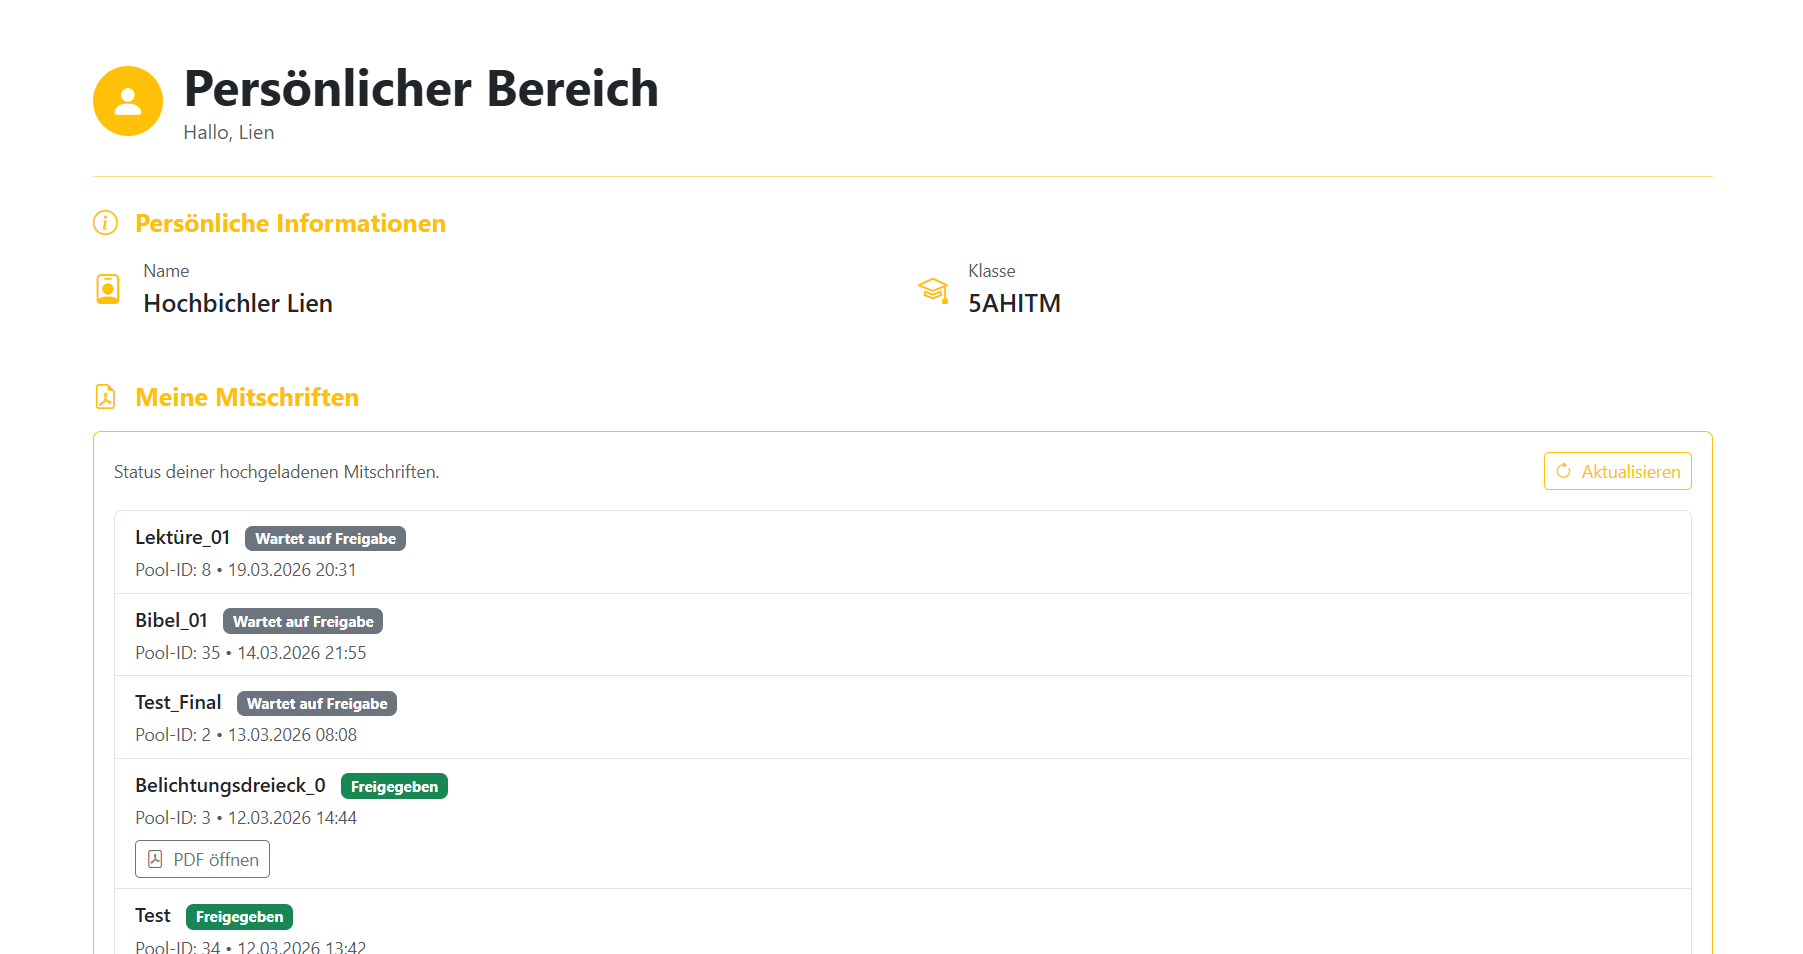
\includegraphics[width=0.9\textwidth]{pics/ab7.png}
    \caption{Persönlicher Bereich: Schüler:in}
    \label{fig:persoenlicher-bereich-schueler}
\end{figure}

Im Bereich \textit{Meine Mitschriften} wird für jede hochgeladene 
Mitschrift der aktuelle Status angezeigt, entweder \textit{Wartet auf 
Freigabe} oder \textit{Freigegeben}. Freigegebene Mitschriften können 
direkt als PDF geöffnet werden.

Zusätzlich gibt es einen Benachrichtigungsbereich, in dem Schüler:innen 
über Freigaben oder Ablehnungen ihrer Mitschriften informiert werden.

\begin{figure}[H]
    \centering
    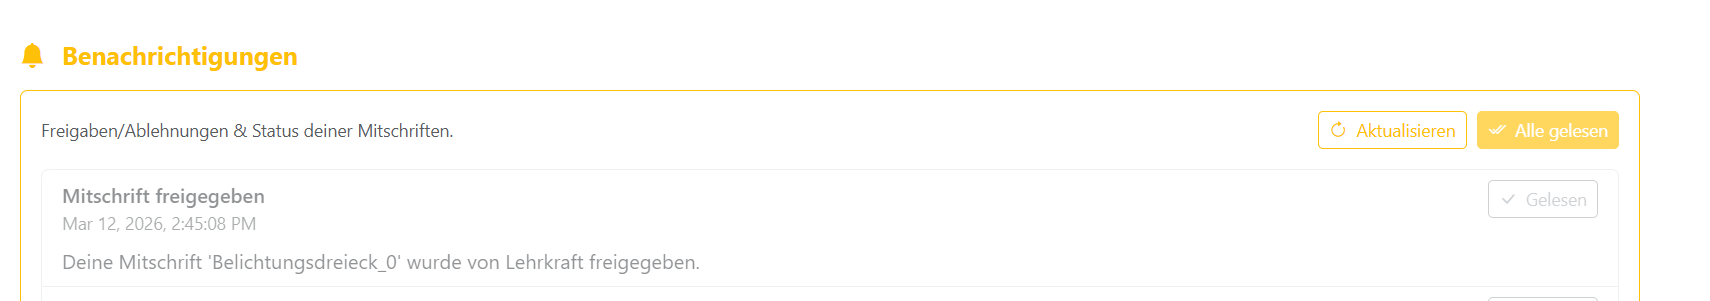
\includegraphics[width=0.9\textwidth]{pics/ab8.png}
    \caption{Benachrichtigungen im persönlichen Bereich}
    \label{fig:benachrichtigungen}
\end{figure}

\paragraph{Ansicht als Lehrkraft}

Lehrkräfte sehen dieselben Informationen wie Schüler:innen, haben 
jedoch zusätzlich Zugriff auf den Button \textit{„Fragen genehmigen"}, 
über den sie zur Freigabeverwaltung gelangen und dort eingereichte 
Fragen von Schüler:innen prüfen können.

\begin{figure}[H]
    \centering
    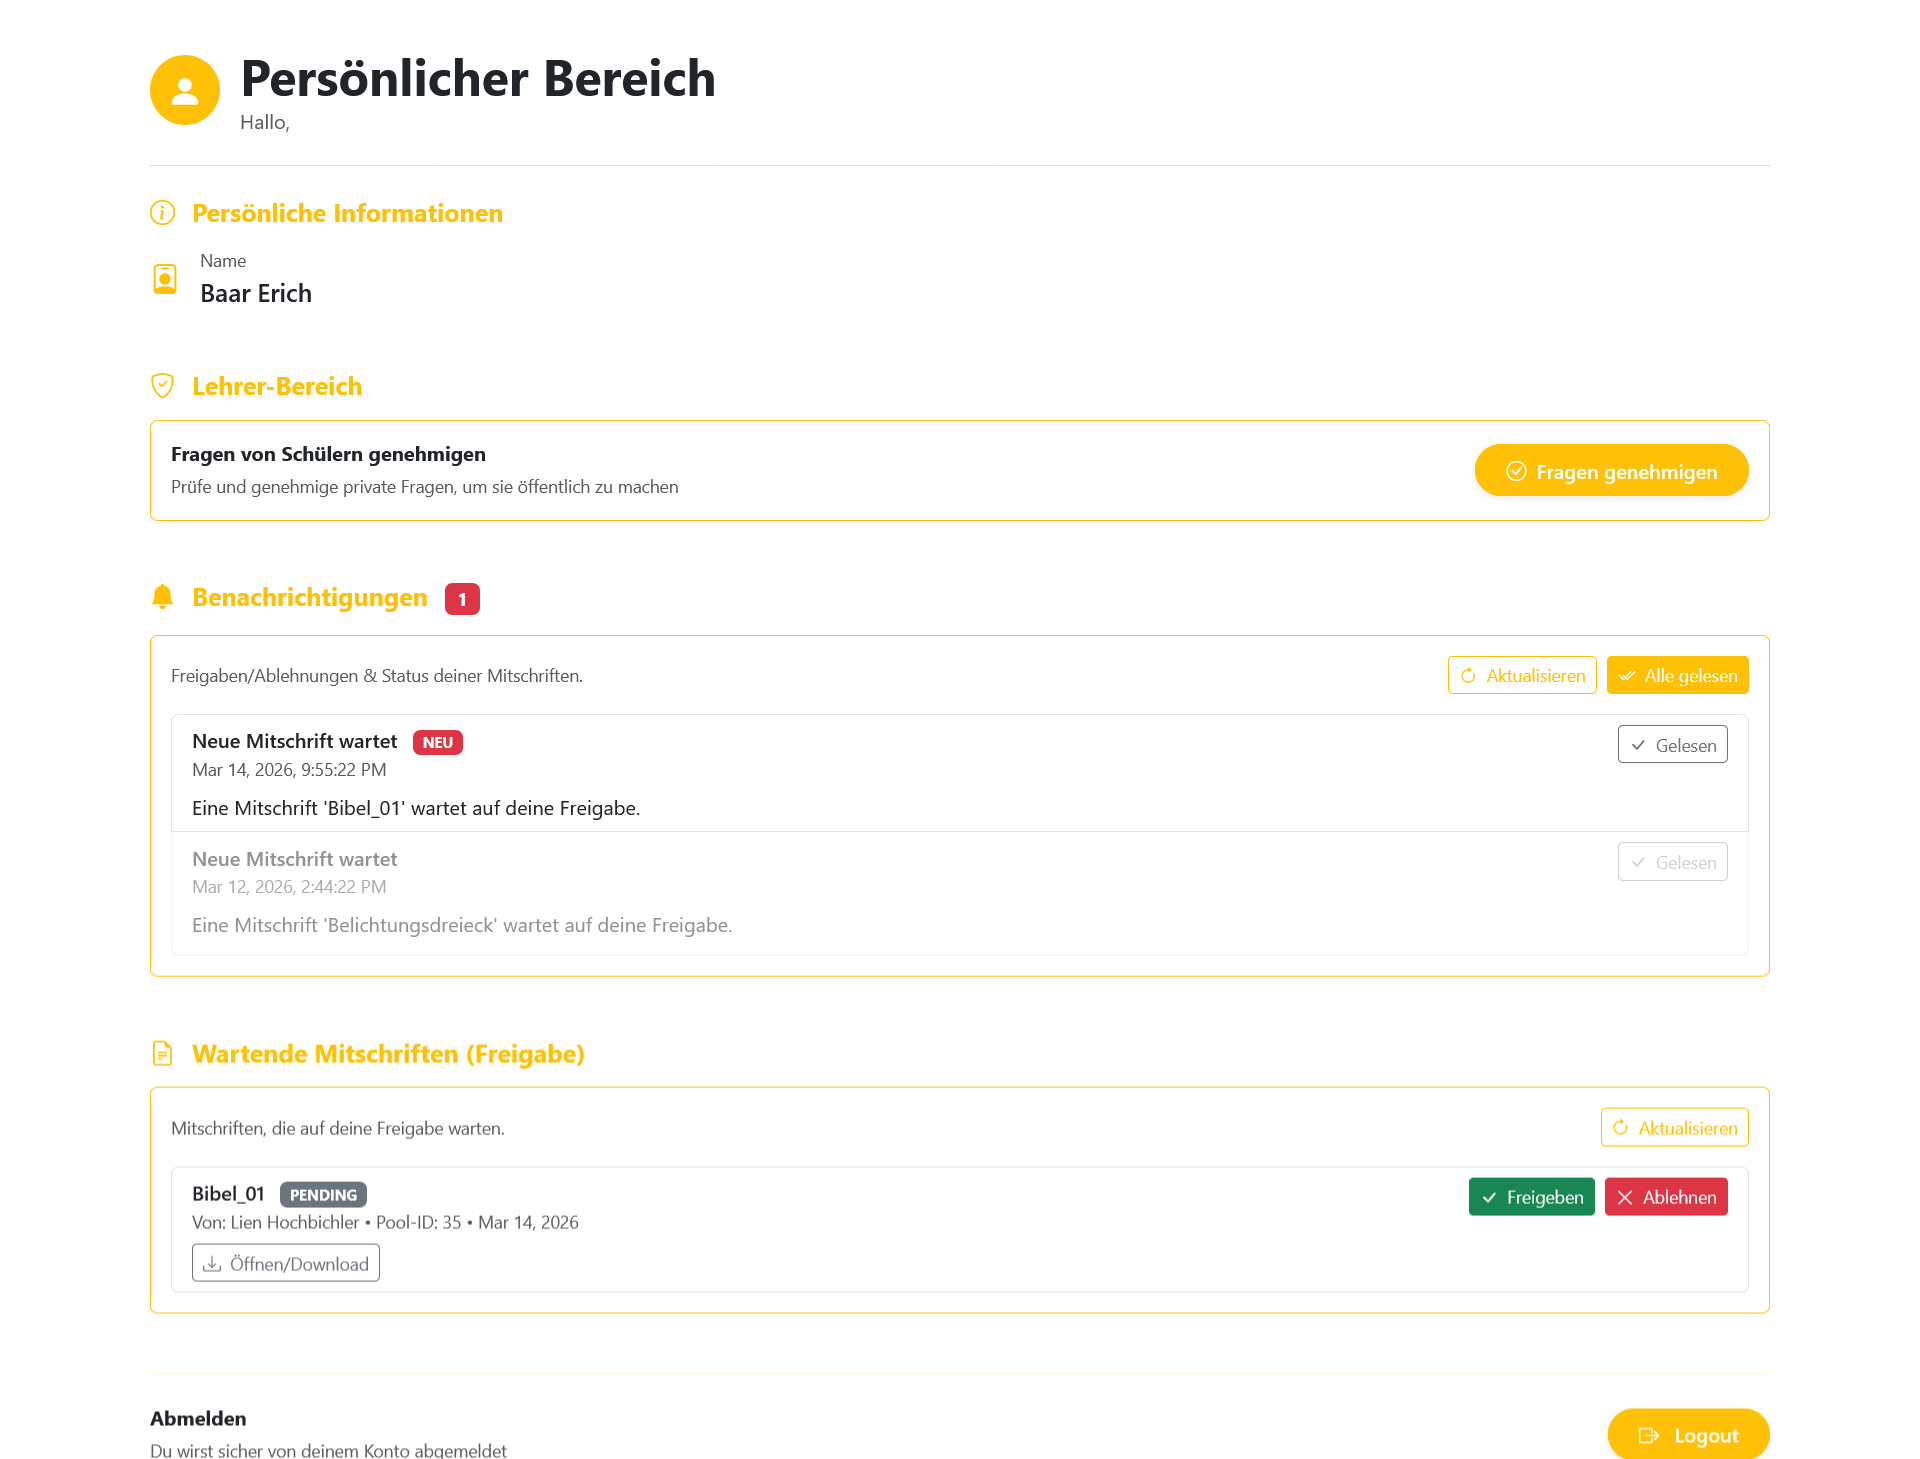
\includegraphics[width=0.9\textwidth]{pics/personal_teacher_view.png}
    \caption{Persönlicher Bereich: Lehrkraft}
    \label{fig:benachrichtigungen-lehrkraft}
\end{figure}

\subsection{Freigabeprozess}

Der Freigabeprozess stellt sicher, dass nur geprüfte Inhalte 
öffentlich sichtbar sind. Abbildung~\ref{fig:freigabe-prozess} 
zeigt den genauen Ablauf.

\begin{figure}[H]
    \centering
    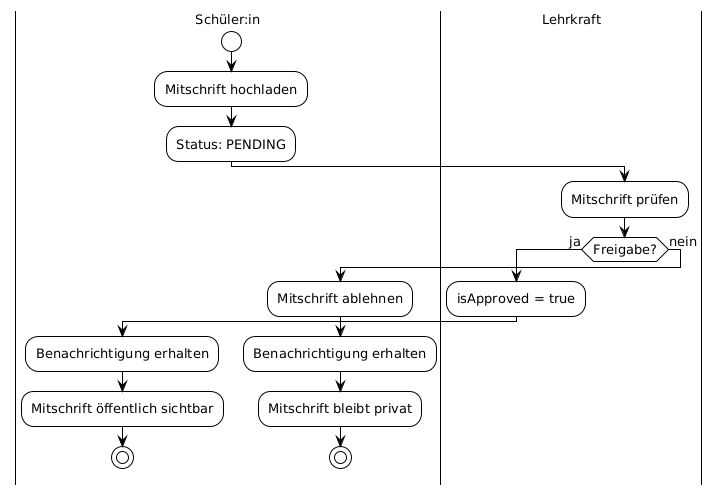
\includegraphics[width=0.75\textwidth]{pics/usecase_mitschirftenUpload.png}
    \caption{Freigabeprozess für Mitschriften}
    \label{fig:freigabe-prozess}
\end{figure}

Sobald eine Schüler:in eine Mitschrift hochlädt, bekommt diese 
automatisch den Status \textit{PENDING}. Die Mitschrift ist in 
diesem Zustand nur für die Ersteller:in selbst sichtbar. Die 
zuständige Lehrkraft sieht alle ausstehenden Mitschriften in 
ihrem persönlichen Bereich und kann diese einzeln prüfen.

Hat die Lehrkraft die Mitschrift geprüft, gibt es zwei 
Möglichkeiten. Entweder wird die Mitschrift freigegeben, 
womit \texttt{approved} in der meta.json auf \texttt{true} 
gesetzt wird und die Mitschrift ab sofort für alle Nutzer:innen 
sichtbar ist. Oder die Lehrkraft lehnt die Mitschrift ab, 
zum Beispiel weil der Inhalt fehlerhaft oder unvollständig ist. 
In beiden Fällen erhält die Schüler:in eine Benachrichtigung 
im persönlichen Bereich.

In der aktuellen Implementierung ist eine Freigabe endgültig 
und kann nicht rückgängig gemacht werden. Eine abgelehnte 
Mitschrift wird vollständig vom Server gelöscht. Für eine 
zukünftige Erweiterung wäre es denkbar, einen 
\texttt{approvedAt} Zeitstempel sowie eine vollständige 
Statushistorie einzuführen, die jede Änderung nachvollziehbar 
dokumentiert. Dies würde jedoch ein eigenes 
\texttt{ApprovalHistory} Entity im Datenmodell erfordern.